\mychapter{Características de um Rede Multi VANTs}
\label{Cap:Requisitos}

As redes multi VANTs são uma evolução do sistema de comunicação formado por apenas um VANT e a base de controle, onde toda a troca de informações é realizada através de um \emph{link} entre as duas partes do sistema e, caso esse \emph{link} fosse interrompido por algum motivo, toda a comunicação seria impossibilitada. A rede multi VANTs é, então, proposta com intuito de aumentar o alcance e a confiabilidade do sistema através da adição de novos nós.

\cite{gupta2015survey} apresenta algumas das característica de uma rede multi VANTs comparando-as a solução baseada em um único VANT, sendo elas:
\begin{itemize}
\item Escalabilidade
\item Capacidade de Sobrevivência
\item Velocidade da Missão
\item Complexidade do Controle
\item Economia de Energia
\end{itemize} 

\section{Escalabilidade}

Por definição uma rede multi VANTs é uma versão escalada da solução composta por um único VANT mais base de controle. Dessa forma, a adição de nós se torna uma operação comum a uma rede multi VANTs tornando-a uma solução escalável que pode variar o tamanho e, consequentemente, o alcance da rede dada as necessidades especificas da missão.

\section{Capacidade de Sobrevivência}

Como mencionado anteriormente, em uma solução formada por um único VANT mais base de controle, a rede é composta por apenas um \emph{link} e, caso esse seja interrompido, a comunicação entre esses dois nós será perdida. No entanto, dado que uma rede multi VANTs será formada múltiplos nós e \emph{links}, em caso da perda de um nó a rede pode se reorganizar e garantir a sobrevivência da rede como um todo. 

Por exemplo, em uma rede composta por quatro nós em topologia \emph{mesh} como mostra a fig. \ref{fig:perdaNo}, no caso de falha do nó B, a comunicação entre os nós entre os nós A e D poderá ser feita através do nó C, garantindo assim a sobrevivência da rede. 

\begin{figure} 
\center
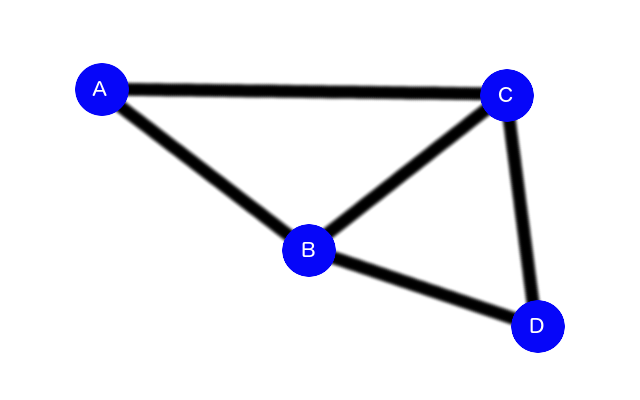
\includegraphics[width=0.7\textwidth]{perdaNo.png}
\caption{Exemplo de topologia de uma rede multi VANTs composta por 4 nós.} 
\label{fig:perdaNo}
\end{figure} 

\section{Velocidade da Missão}

A velocidade de realização de uma determinada missão será proporcional ao tamanho da rede multi VANT, quanto maior a quantidade de VANTs em uma determinada rede a ser utilizada para executar uma missão de varredura de área, menor será o tempo da missão. Por exemplo, pode-se dividir a área a ser varrida em sub-áreas que serão varridas simultaneamente, alocando cada VANT disponíveis para a missão a uma sub-área diferente. Por outro lado, a adição de um nó a uma rede resultará no aumento do custo da missão. Dessa forma, é importante analisar os benefícios do aumento de uma rede multi VANTs do ponto de vista financeiro. 

\section{Complexidade do Controle}

A complexidade do controle de uma rede composta por apenas um VANT e uma base de controle é baixa quando comparado ao cenário de uma rede multi VANTs. Quanto maior a quantidade de nós em uma rede maior será o custo computacional para controlar os nós e determinar os caminhos para realização da comunicação entre eles.

Outro ponto que aumente ainda mais essa complexidade é a frequente mudança de topologia da rede, seja causada pela movimentação rápida dos nós, que se dá nas três dimensões, ou pela perda de nós devido a problemas de funcionamento ou fim da carga da bateria que alimenta o VANT.

\section{Economia de Energia}

Como VANTs possuem fonte de alimentação limitada, é importante garantir que rede funcione da forma mais eficiente possível quanto ao consumo de energia, de tal forma que os nós possam permanecer ativos na rede pelo máximo de tempo possível. Caso a rede de comunicação consuma muita energia dos VANTs, será necessário a substituição de nós durante a execução de uma missão o que, consequentemente, aumentará o tempo necessário para a realização da mesma.\\

As características discutidas nesta sessão servirão de base para produção do protocolo de testes e, por fim, desenvolvimento da arquitetura de rede a ser implementada futuramente. 